\documentclass{standalone}

\input{../colours.tex.preamble}
\input{../tikz.tex.preamble}

\begin{document}
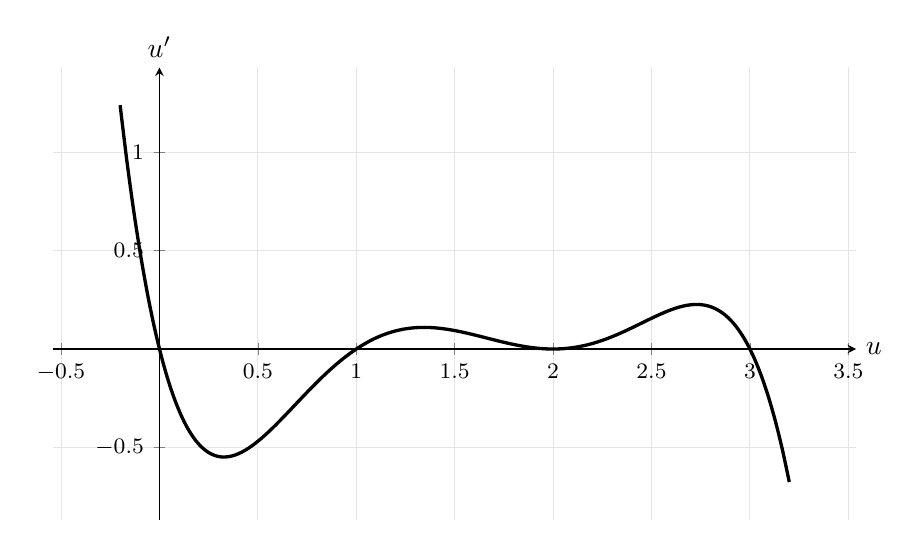
\begin{tikzpicture}[define rgb/.code={\definecolor{mycolor}{RGB}{#1}}, rgb color/.style={define rgb={#1},mycolor}]
  \begin{axis}[
    height=4in,
    axis lines = middle, % boxed, middle
    % axis on top,
    axis equal image,
    %
    % domain and range
    %
    % xmin={}, xmax={},
    % ymin={}, ymax={},
    enlargelimits=true,
    %
    % axis labels
    %
    xlabel={\(u\)}, xlabel style={anchor=west},
    ylabel={\(u'\)}, ylabel style={anchor=south},
    label style={at={(ticklabel* cs:1)}},
    %
    % ticks
    %
    % xtick={}, xticklabels={},
    % ytick={}, yticklabels={},
    ticklabel style={font=\footnotesize},
    %
    % grid
    % none, major, minor, both
    grid=major, grid style={gray!20},
    % minor tick num=1, 
    % minor grid style={gray!20},
    % 
    % plot parameters
    %
    smooth, samples=100, no markers,
    % xtick={}, xticklabel={},
    % ytick={}, yticklabel={}
    ]

    % \foreach \p in {0.1, 0.2, ..., 0.9} {
    %   \addplot[main, thick] {1 / ( 1 + ( (1 -  \p) /  \p ) * exp( -x ) )};
    % }
    % \foreach \p in {1.1, 1.2, ..., 1.5} {
    %   \addplot[supp, thick] {1 / ( 1 + ( (1 -  \p) /  \p ) * exp( -x ) )};
    % }
    \addplot[very thick, domain=-0.2:3.2] {x*(x-1)*(2-x)^2*(1-x/3)};
  \end{axis}
\end{tikzpicture}
\end{document}
